\documentclass[12pt, a4paper]{article}
\usepackage[utf8]{inputenc}
\usepackage{amsmath}
\usepackage{amsfonts}
\usepackage{amsthm}
\usepackage{graphicx}
\usepackage{parskip}
\usepackage{hyperref}
\usepackage{fancyhdr}
\usepackage{lastpage}
\usepackage{tikz}
\usepackage{float}
\usepackage{listings}
\usepackage{color}
\usepackage{caption}
\usepackage[acronym]{glossaries}
\usepackage[nottoc]{tocbibind}
\usepackage[cache=false]{minted}
\usemintedstyle{default}
\newminted{haskell}{frame=lines,framerule=2pt}
\graphicspath{{./images/}}

\tikzstyle{bag} = [align=center]

\title{%
      Homework 3 \\
      Experimental Comparison between KDTrees vs. Locality Sensitivity Hashing
}
\author{%
  Juan Pablo Royo Sales \\
  \small{Universitat Politècnica de Catalunya}
}
\date\today

\pagestyle{fancy}
\fancyhf{}
\fancyhead[C]{}
\fancyhead[R]{Juan Pablo Royo Sales - UPC MIRI}
\fancyhead[L]{ADM - Homework 3}
\fancyfoot[L,C]{}
\fancyfoot[R]{Page \thepage{} of \pageref{LastPage}}
\setlength{\headheight}{15pt}
\renewcommand{\headrulewidth}{0.4pt}
\renewcommand{\footrulewidth}{0.4pt}

\makeglossaries

\newacronym{lsh}{LSH}{Locality Sensitivity Hashing}
\newacronym{kdt}{KDTree}{KDTrees}
\newacronym{nns}{NNS}{Nearest Neighbor Search}
\newacronym{haskell}{Haskell}{Haskell Programming Language}
\newacronym{kde}{KDE}{Kernel Density Estimate}
\newacronym{lrm}{LRM}{Linear Regression Model}
\newacronym{cod}{CoD}{Curse of dimensionality}

\begin{document}

\maketitle

\section{Introduction}\label{sec:intro}
In this work, I am going to show the experimental results of comparing \acrfull{lsh} vs. \acrfull{kdt} for doing \acrfull{nns} algorithm as a good predictor.

In previous works \cite{hmw1} and \cite{hmw2} I've done a deep analysis on how this Data Structures work in order to achieve good asymptotic cost for doing \acrshort{nns} and predict values.

In this work I have done an implementation of both Data Structures in Haskell \acrfull{haskell}.

In the following sections I am going to describe where it can be found each source of information and code as well as the experiments run and the results.

\section{Asset organization}
Please check the appendix~\ref{apx:org} to see how the different assets are organized, how to run the experiment, and so on.

\section{Data Source}
\subsection{Static Data}
The data source used for this experiment is the \textbf{Transactional Grocery Store} data accorded with the teacher that can be found in~\ref{apx:data}.

I have chosen this data in agreement with the teacher because we want to experiment on high dimensional transactional data.

This data source contains \textbf{1000} records of transactional data with at most \textbf{15} dimensions.

The data set is divided into:

\begin{itemize}
  \item 800 Rows of Training Data
  \item 200 Rows of Testing Data
\end{itemize}

\subsection{Randomized Data}\label{sub:sec:random:data}
For randomization experiments, I am generating $100000$ records with 15 dimensions each of positive integer values each.

For that I am using a \acrshort{haskell} library called QuickCheck \cite{QuickCheck}.

After generating the points I am splitting up in Training and Test Data Set of equal size $50000$

   \begin{listing}[H]
    \inputminted[firstline=11, lastline=15]{haskell}{../app/random/Main.hs}
    \caption{Extracted from source code app/random/Main.hs}
    \label{src:main:random}
   \end{listing}



\subsection{Sanitizing Data}
Since the data is not structured and each record contains different dimension we need to sanitize somehow in order to be able to feed the algorithm for further processing.

In the case of \acrshort{lsh} implementation, I don't need this sanitation because my implementation works on set of value hashing, so different combinations of unstructured record which are similar will lead to the same hash bucket.

On the other hand, in the case of \acrshort{kdt}, I am going to need to sanitize this data because since \acrshort{kdt} is a multidimensional data structure, all the dimensional points are need to be represented in a structured way.

For that reason I have done the following sanitation:

\begin{itemize}
  \item Having different records of that like:

    \inputminted[firstline=2, lastline=12]{text}{../input/data.in}

  \item I took all the different possible dimensional labels
    \begin{listing}[H]
    \inputminted[firstline=91, lastline=108]{haskell}{../src/IO/Data.hs}
    \caption{Extracted from source code src/IO/Data.hs}
    \label{src:io:data:1}
    \end{listing}

  \item With for each record I create a dimensional point of 15 dimension with Bits values that indicates $1$ if the dimension is present in the record, $0$ otherwise.
    \begin{listing}[H]
    \inputminted[firstline=72, lastline=82]{haskell}{../src/IO/Data.hs}
    \caption{Extracted from source code src/IO/Data.hs}
    \label{src:io:data:2}
    \end{listing}

\end{itemize}

\section{Experiments Details}
As I pointed out in the Introduction section~\ref{sec:intro}, I have already analyzed theoretical properties of these two Data Structures in the previous homework. Therefore, the main goal of this work is to focus in the experimental comparison.

In order to do that, I have defined 3(\textbf{three}) experiments.

\begin{itemize}
  \item \textbf{Benchmark}
  \item \textbf{Qualitative}
  \item \textbf{Randomized Benchmark}
\end{itemize}

\subsection{Benchmark}\label{sub:sec:bench}
This experiment consist in measuring and comparing the empirical performance on both data structures. For that I have used a very well known \acrshort{haskell} library \cite{criterion}.

Basically this library run several samples of the same process to take statistical analysis of the running time of the process. With that statistical information it builds a \acrfull{kde} graphic and a \acrfull{lrm}.

The benchmarking experiments are going to be focus on the following comparisons:

\begin{itemize}
  \item Running time of loading Training Data Set on \acrshort{lsh}
  \item Running time of loading Training Data Set on \acrshort{kdt}
  \item Running time of performing \acrshort{nns} on each Test Data Set on \acrshort{lsh}
  \item Running time of performing \acrshort{nns} on each Test Data Set on \acrshort{kdt}
\end{itemize}

\subsection{Qualitative}
Qualitative analysis is basically load the training data, and after that for each row of the Testing Data Set, run \acrshort{nns} in order to see and analyze each result.

\subsection{Randomized Benchmark}\label{sub:sec:exp:random}
Randomized Benchmark is the same kind of experiment as Benchmark~\ref{sub:sec:bench} but the difference is that I am using randomized generated data to train and search in the model.

This experiment I have done in order to test the performance of the Data Structures with a lot of data since $1000$ records it is not too much.

In order to see details about randomized data generation check subsection~\ref{sub:sec:random:data}

\section{Results}
\subsection{Benchmark}
This are the graphics after running the benchmark analysis.

\subsubsection{Overview}
In the overview analysis, in terms of time we can appreciate that in general training data, which is loading into the structure, is much more efficient in \acrshort{lsh} rather than in \acrshort{kdt}.

On the other hand we can see that searching is more efficient on \acrshort{kdt} in terms of time but the difference is in term of $\mu s$ which is not so significant, but lets analyze this in deep later in following section.

\begin{minipage}[t]{\linewidth}
  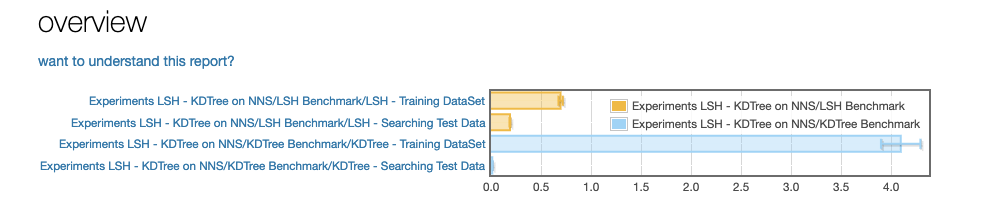
\includegraphics[width=\textwidth]{bench_overview}
  \captionsetup{type=figure}
  \captionof{figure}{Overview Benchmark}
  \label{fig:bench_overview}
\end{minipage}


\subsubsection{Training Data}

\begin{itemize}
\item \textbf{LSH Training}
As we can see in the following graph we can appreciate that Data training or load in the case of \acrshort{lsh} behaves normally distributed around $696 \mu s$ as the mean indicates.

On the other hand the \textbf{Outlyings} has only an impact of $21.9\%$ only which indicates that the program behaves equal across the samples.

We can appreciate also a good fit of $0.996$, so the distribution is not too noisy.

\begin{minipage}[t]{\linewidth}
  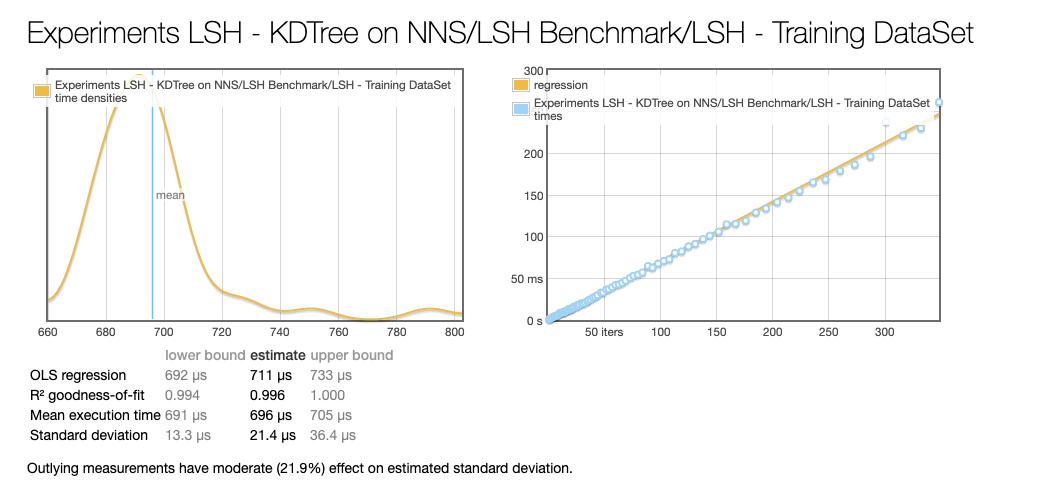
\includegraphics[width=\textwidth]{bench_lsh_load_training_ds}
  \captionsetup{type=figure}
  \captionof{figure}{LSH Training Data - Benchmark}
  \label{fig:bench_lsh_load_training_ds}
\end{minipage}

Regarding the \acrshort{lrm} build by the tool we can see also how the points are near the line which indicates that we can estimate with a good precision the next run of the training, giving us a good program that we can predict how is going to run.

\item \textbf{KDTree Training}
As I can show in the Overview section, training is taking more time for \acrshort{kdt} but for obvious reason of the structure. Inserting in a Hash Table takes $\theta(1)$ time and in a Balance Tree as \acrshort{kdt} is $\theta(\log{n})$ as I have describe in the previous works.

The \textbf{Outlyings} here are affecting more and it seems that across different samples the tree is behaving slightly different, but not so much.

\begin{minipage}[t]{\linewidth}
  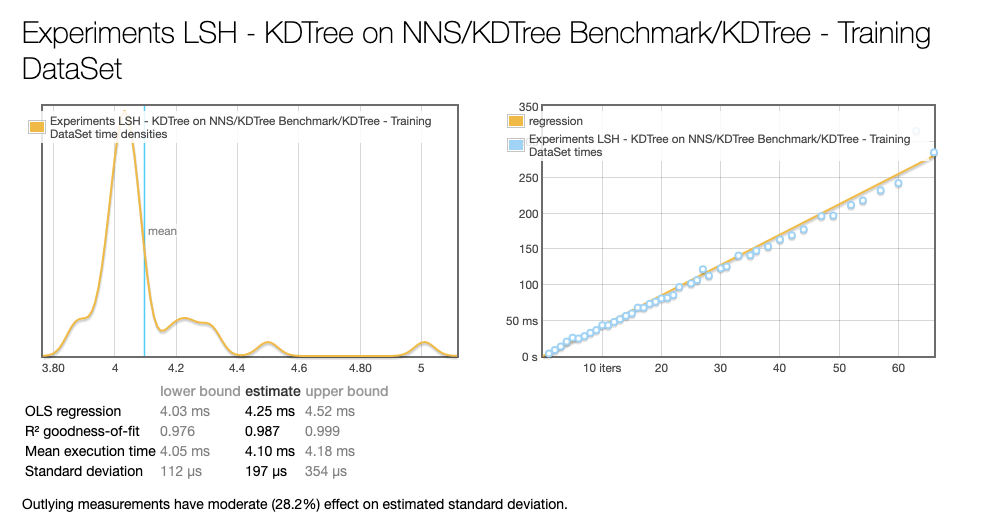
\includegraphics[width=\textwidth]{bench_kdt_load_training_ds}
  \captionsetup{type=figure}
  \captionof{figure}{KDTree Training Data - Benchmark}
  \label{fig:bench_kdt_load_training_ds}
\end{minipage}

The fitting of the model is also good in this case with $0.998$ as estimate vale, and the \acrshort{lrm} also good for predicting runs.

\end{itemize}

\subsubsection{NNS Test Data}\label{sub:sub:sec:test:results}
Lets analyze \acrshort{nns} algorithm for predicting points with the Test Data Set.

\begin{itemize}
\item \textbf{LSH NNS}
Regarding searching of points It can be appreciated that in this case the results are also quite good in terms of Fitting with a Good fit of $0.998$, time $191 \mu s$ and also distribution of the samples with only a $18.2\%$ effect of \textbf{Outlyings}.

\begin{minipage}[t]{\linewidth}
  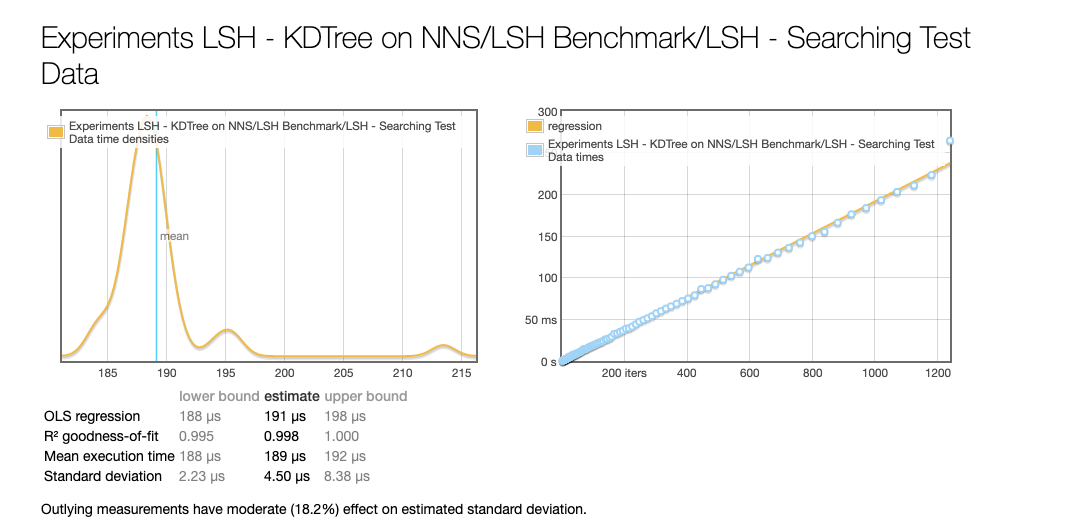
\includegraphics[width=\textwidth]{bench_lsh_nns_test_ds}
  \captionsetup{type=figure}
  \captionof{figure}{LSH NNS Test Data - Benchmark}
  \label{fig:bench_lsh_nns_test_ds}
\end{minipage}

Also the \acrshort{lrm} indicates a good prediction on next searches and how the algorithm is going to perform in that sense.

\item \textbf{KDTree NNS}
Regarding \acrshort{kdt} it can be appreciated here why it is taking much less time to do an \acrshort{nns} rather than \acrshort{lsh}, and that is because the effect of \textbf{Outliers} is high with $89.2\%$, therefore the sample is too much noisy and the algorithm is not behaving stable as expected.

\begin{minipage}[t]{\linewidth}
  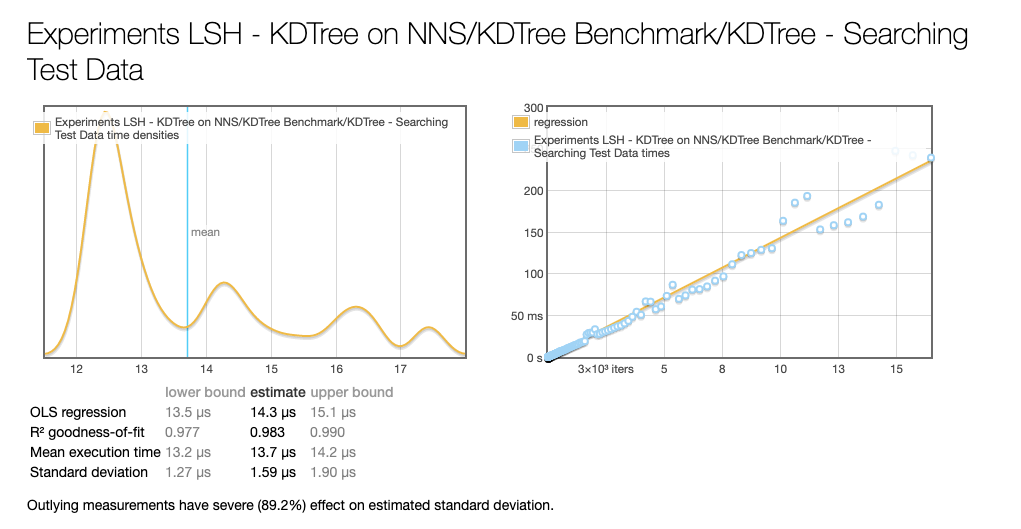
\includegraphics[width=\textwidth]{bench_kdt_nns_test_ds}
  \captionsetup{type=figure}
  \captionof{figure}{KDTree NNS Test Data - Benchmark}
  \label{fig:bench_kdt_nns_test_ds}
\end{minipage}

As I have stated in my previous deliverable \cite{hmw2}, \acrshort{kdt} suffers from what is called the \textbf{\acrfull{cod}}, and we are dealing with $15$ dimensions here and for the data structure is complicate to handle that and the cost of searching increase more than linear.

This can be seen also in the \acrshort{lrm} where we can the see the pints outlying the line.
\end{itemize}

\subsection{Qualitative Results}\label{sub:sec:qual:results}
As you can see on the appendix~\ref{apx:reports}, the results of this analysis can be found in \mintinline{bash}{output} folder and are the files with \mintinline{bash}{.csv} extension.

Also the summary which is the following

\begin{listing}[H]
\inputminted{text}{../output/data_summary_1587016424.out}
\caption{Summary Qualitative Analysis}
\label{output:summary}
\end{listing}

As we can appreciate the level of successful predictions in \acrshort{lsh} is much more higher than \acrshort{kdt}.

This could be explain because of what i stated in the previous section that \acrshort{kdt} suffers from \acrshort{cod}. The real predictions that this kind of structure can do is very low compared with \acrshort{lsh}.

\subsection{Randomized Benchmark}\label{sub:sec:results:random}
You can check setup of this experiment in~\ref{sub:sec:exp:random}.

In the case of randomized Benchmark we have found the following results:

\begin{itemize}
  \item \textbf{LSH}:

    As it can be appreciated in the following graph, training with much more data decreased the time spent on loading the Hashtable but we can appreciate that there is no \textbf{outliers} affecting the distribution and the structure behave stable across run.

\begin{minipage}[t]{\linewidth}
  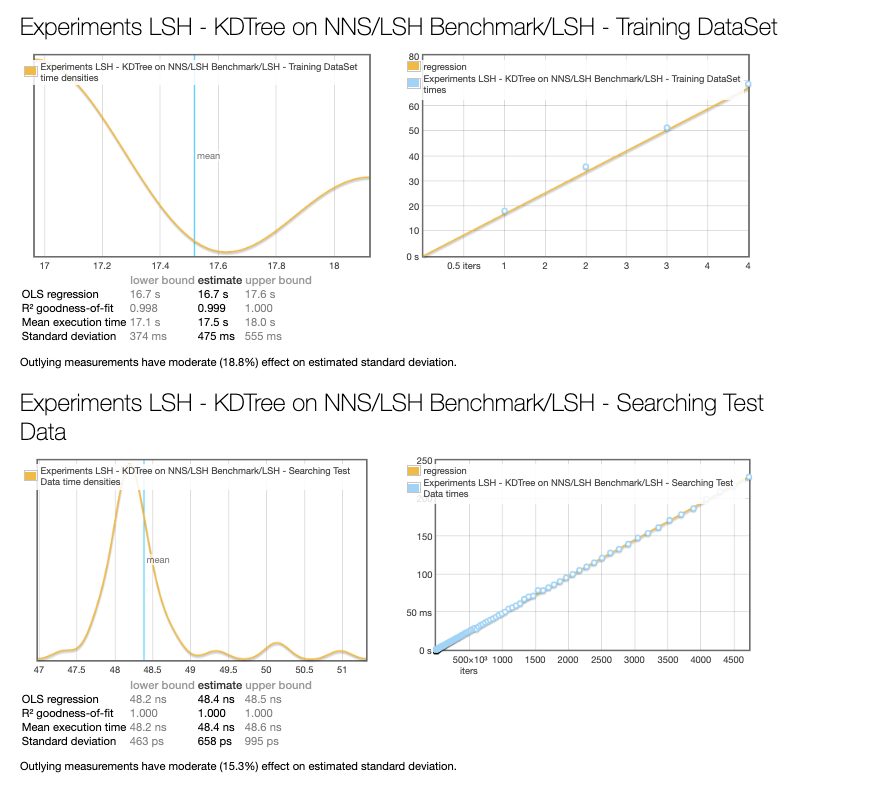
\includegraphics[width=\textwidth]{random_bench_lsh}
  \captionsetup{type=figure}
  \captionof{figure}{Randomized LSH - Benchmark}
  \label{fig:random_bench_lsh}
\end{minipage}

Also in searching we can appreciate extremely good results in terms of time, distribution and Good fit.

  \item \textbf{KDTree}:

In the case of this structure we are seeing the same behavior that with the regular benchmark analysis.

It is more costly to load and train the structure because of the amount of records, but on searching we start seeing the effect of \textbf{outliers} as we experience in the regular benchmark results with a high percentage of them $74.4\%$.

 \begin{minipage}[t]{\linewidth}
  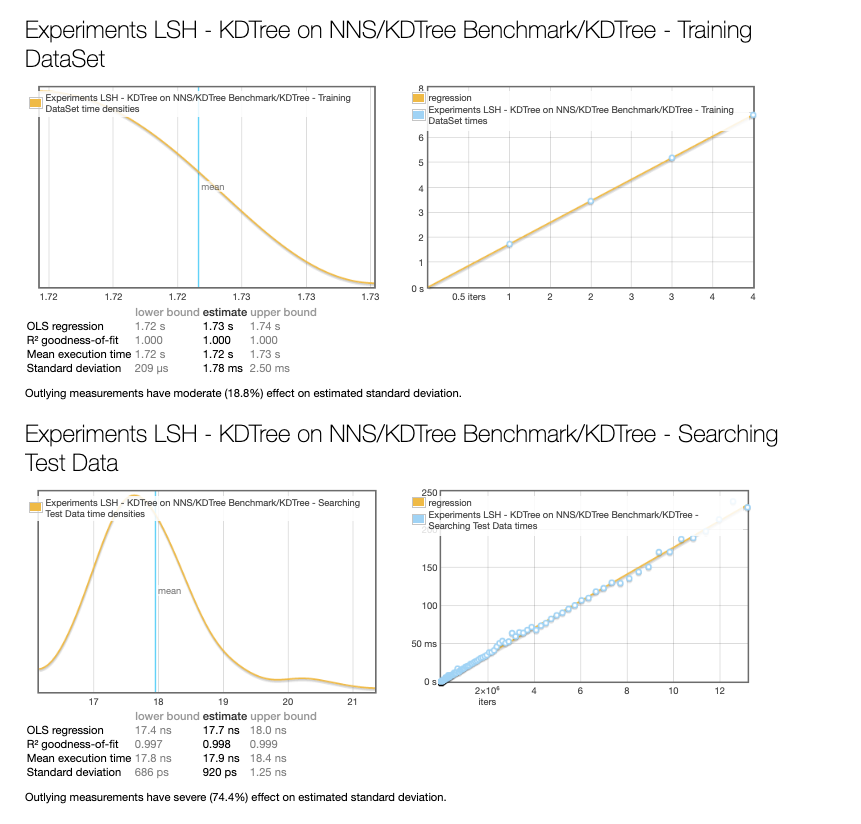
\includegraphics[width=\textwidth]{random_bench_kdt}
  \captionsetup{type=figure}
  \captionof{figure}{Randomized KDTree - Benchmark}
  \label{fig:random_bench_kdt}
 \end{minipage}


\end{itemize}

In general both structure follow the same pattern for randomized data than with specific transactional data, which indicates that there is empirical evidence that show us both structure are deterministic in their behavior.

\section{Conclusions}
In conclusion we have shown through this experimental analysis that \textbf{\acrlong{lsh}} behaves better for predicting and dealing with high dimensions, rather than \textbf{\acrlong{kdt}}.

This can be seen on results here~\ref{sub:sub:sec:test:results} very clearly and also if we randomized data here~\ref{sub:sec:results:random}.

All the results obtain through the experiments are showing that the theoretical difference presented in \cite{hmw1} and \cite{hmw2} can be proved empirically.

Dealing with higher dimensional data could lead to inefficient structures if it is required to perform Ranged Queries or \acrlong{nns} algorithms for predictions. Having clever structures and algorithms like \acrfull{lsh} has shown that is an excellent alternative to deal with this problem.

\bibliographystyle{alpha}
\bibliography{report}

\printglossary[type=\acronymtype]

\appendix\label{apx:org}
\section{Haskell}
\subsection{Source Code}
In the source code there are 2 folders with code:

\begin{itemize}
  \item \textbf{app}: Which contains 3 programs with the 3 executables source code file. Here we can find:
    \begin{itemize}
      \item \textbf{\mintinline{haskell}{app/bench/Main.hs}}: It is the main entry point that run the Benchmark analysis in both Data Structures.
      \item \textbf{\mintinline{haskell}{app/data/Main.hs}}: It is the main entry point that run the A Qualitative analysis in both Data Structures to see what is the output on each case.
      \item \textbf{\mintinline{haskell}{app/random/Main.hs}}: It is the main entry point that run a Benchmark but based on Random generate data in both Data Structures.
    \end{itemize}
  \item \textbf{src}: Contains the implementation source code of the Data Structures.
    \begin{itemize}
      \item \textbf{\mintinline{haskell}{src/Experiments.hs}}: It contains the different experiment run.
      \item \textbf{\mintinline{haskell}{src/Data/LSH/LSH.hs}}: \acrshort{lsh} Implementation.
      \item \textbf{\mintinline{haskell}{src/Data/Tree/KDTree.hs}}: \acrshort{kdt} Implementation.
      \item \textbf{\mintinline{haskell}{src/Data/Types.hs}}: Usefull types to handle 15 dimensional points.
      \item \textbf{\mintinline{haskell}{src/IO/Data.hs}}: Handle reading dataset from file, sanitizing and transforming to be fed into implementations. Also partition the data between training and test set.
    \end{itemize}

\end{itemize}

\subsection{Run the Code}
All the solution has been coded with \textbf{Stack} \cite{stack} version 2.1.3 or higher. It is a prerequisite to install \textit{stack} for running this code.

\subsubsection{Running Experiments}
In order to run the experiments just do the following in each case.

\begin{itemize}
  \item \textbf{Benchmark Experiment}

\begin{minted}{bash}
stack build
stack exec lsh-kdtree-bench -- --output MY_OUTPUT_FILE.html
\end{minted}

This is going to left an HTML report with the benchmark results in \mintinline{bash}{MY_OUTPUT_FILE.html}

\item \textbf{Randomized Benchmark Experiment}

\begin{minted}{bash}
stack build
stack exec lsh-kdtree-random -- --output MY_OUTPUT_FILE.html
\end{minted}

This is going to left an HTML report with the randomized benchmark results in \mintinline{bash}{MY_OUTPUT_FILE.html}


\item \textbf{Qualitative Data Experiment}

\begin{minted}{bash}
stack build
stack exec lsh-kdtree-data
\end{minted}

This is going to print a summarized result, but it is going to left \textbf{csv} files under \mintinline{haskell}{output} directory with a timestamp suffix to identified the run, where you can find that for every tested data case what is the \acrshort{nns} result.

\end{itemize}

\section{Data Source - Input}\label{apx:data}
Input data or Data Source is being store under \mintinline{haskell}{input} folder.

\section{Generated Outputs}\label{apx:reports}
All the Generated Outputs that has been used to build this document are under \mintinline{haskell}{output} folder.

\begin{itemize}
  \item \textbf{html}: HTML files on this folder are Benchmark graphics and report generated by \cite{criterion} tool.
  \item \textbf{csv}: CSV files on this folder have been generated by Qualitative analysis and contains for each searched value the response of the algorithm.
  \item \textbf{out}: Files whose extension is \mintinline{bash}{.out} is a summary of the successful findings in Qualitative analysis.
\end{itemize}

\section{Report PDF Document}
This report document is under \mintinline{haskell}{doc} folder alongside images that are embedded in this report.


\end{document}

